\documentclass[a4paper,11pt]{article}
\usepackage[T1]{fontenc}
\usepackage[utf8]{inputenc}
\usepackage{lmodern}
\usepackage{hyperref}
\usepackage{graphicx}
\usepackage{rotating}
\usepackage{listings}
\usepackage{color}
\usepackage{listings}
\usepackage{pdfpages}

\title{Advanced Algorithms - part 2 (exc 4-6) by}
\author{Arash Rouhani (rarash@student.chalmers.se) - 901117-1213}


\begin{document}

\maketitle

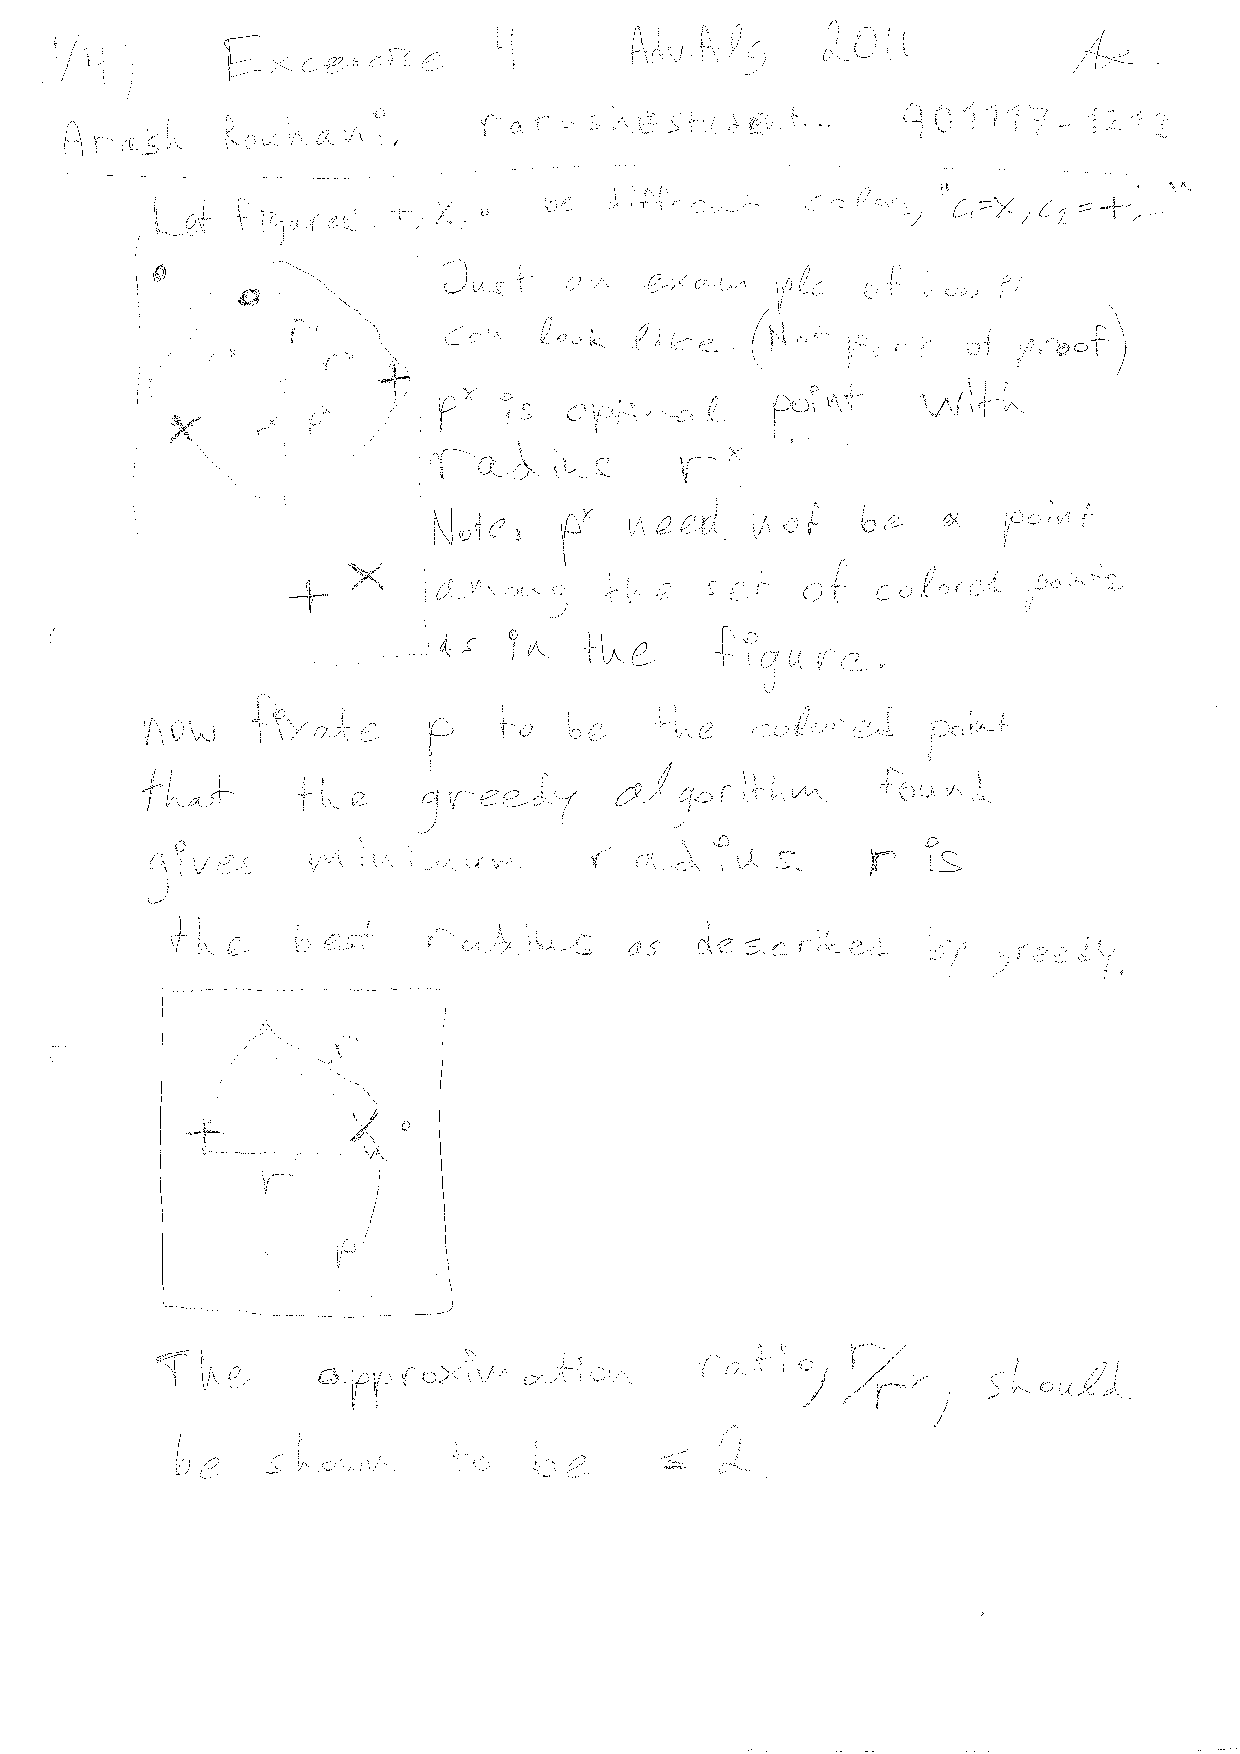
\includepdf[pages=-]{20111105191330882.pdf}

\section{Weigthed Hitting Set}

$A$ is our set with $n$ elements (our nodes), having weights $w_i$.
We have $m$ subsets $B_j$, $|B_j| \leq b$. An answer $S$ will have cost $w(S)$.
I won't repeat the whole problem formulation.

We follow the given hint, so we make an extended version of
the pricing analogy, basically, each subset pays for contained nodes.
And fair prices is held when $\forall i, \quad \sum_{i \in B_j} p_j \leq w_i$.
So each $B_j$ has its price $p_j$.

\subsection{Algorithm}

A node is tight when $\forall i, \quad \sum_{i \in B_j} p_j = w_i$.
Loops over all $j$ in any order. Increase $p_j$ as much as possible
without violating fair prices (that is, until one of the nodes are tight).
The answer $S$ is the set of tight nodes.

\subsection{Analysis}

First let's assure that $S$ is a hitting set cover. $S$ must
be a solution by proof of contradiction, let's say that
the subset $B_j$ is left unhit. So will be the case if all nodes in
$B_j$ are non-tight, but that won't happen as the algorithm
was supposed to increase $p_j$ until one of the nodes in $B_j$
became tight.

By definition of the return set $S$ we have
$\forall i \in S, \sum_{i \in B_j} p_j = w_i$.
This gives $ \sum_{i \in S} \sum_{i \in B_j} p_j = w(S)$.
Every price $p_j$ will occur at most $b$ times in the sum
(exactly $b$ times if all $|B_j| = b$ and $S = A$).
So definetly $w(S) \leq b \sum_{all j} p_j$.

Before drawing our last conclusion, we must note that
$\sum_{all j} p_j \leq w(S) $ for \emph{any} solution $S$.
Motivation follows:
If fair prices are held, we have
$\sum_{i \in B_j} p_j \leq w_i$ and in particular
$\sum_{i \in S} \sum_{i \in B_j} p_j \leq w(S)$.
A hitting set have hitten every subset, so surely
$\sum_{all j} p_j \leq \sum_{i \in S} \sum_{i \in B_j} p_j \leq w(S)$

Now we consider $S$ as the greedy solution again.
Given $w(S) \leq b \sum_{all j} p_j$ and $\sum_{all j} p_j \leq w(S)$.
So say the optimum weight is $K=w(S^*)$, of course
$\sum_{all j} p_j \leq K \leq b \sum_{all j} p_j$.
In ideal case $K = \sum_{all j} p_j$,
so we conclude that our greedy won't do worse than $b$
times the optimum value. Done.

\end{document}
